There are currently four seperate main drop downs from the menu bar, these are: File, Edit, View Spectrum Data, and List Mode Data Analysis.
\section{File Menu}
	This menu is primarily used for the loading and saving of calibrated spectrum. The methods are listed below as well as there functions:
		\subsection{Load New Spectrum}
			This will open a pop up, this is seen below in Figure \ref{fig:load_new}. \\
				\begin{figure}[h!]
					\centering
					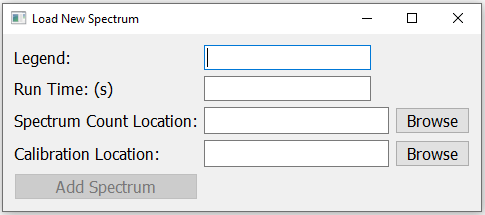
\includegraphics[width=0.7\linewidth]{Load_New.png}
					\caption{GUI to load new spectrum and calibration.}
					\label{fig:load_new}
				\end{figure}
		It expects as input:
				\subsubsection{Legend} 
					The name associated with the calibrated spectrum that will appear in the legend generated during graphing.
				\subsubsection{Run Time(s)}
				 The total run time of the spectrum accumulation. If left blank, it will default to 1.
				\subsubsection{Spectrum Count Location}
				 The absolute path to the file containing the spectrum counts on a per channel basis. Will accept plan text(.txt), comma seperated(.csv), and spectrum files(.spe).
				\subsubsection{Calibration Location}
				 Absolute path to the calibration file generated using the calibrate spectrum feature (discussed in more detail later). This file will be a single column of energy values whose length corresponds to the total number of channels the spectrum was accumulated using. 

		\subsection{Save Spectrum Image}
			This will save a high quality image, 600dpi, to the file name and location entered in the standard windows file explorer that will be brought up upon selection.
		\subsection{Save Spe File}
		Saves the loaded spectrum out to a .spe file format, including the accumulation time. If a non-linear calibration is incorporated, it will fit a linear equation to the data. This is done to ensure an approximate calibration is saved.